%%%%%%%%%%%%%%%%%%%%%%%%%%%%%%%%%%%%%%%%%%%%%%%%%
\chapter{Návrh architektury}
Cílem této kapitoly práce je navrhnout a popsat architekturu, která bude řešit, či umožní budoucí řešení problémů popsaných v kapitole \ref{sec:ana_problems} a vyhoví tak požadavkům na architekturu aplikace definovaným v kapitole \ref{sec:ana_requiremets}.

Tyto požadavky jsou rozděleny na tři skupiny, přičemž řešení požadavků mezi jednotlivými skupinami na jsou na sobě bůďto navzájem nezávislá, nebo je případná závislost explicitně uvedena v následujícím textu.

První jsou problémy způsobené mícháním perzistentní a byznys logiky v rámci serverové části aplikace aplikace, mezi které patří především špatná \textit{modifikovatelnost} aplikace a nízká \textit{viditelnost} interakcí jednotlivých komponent serverové částí aplikace. Také jsou diskutovány dopady těchto omezení na \textit{výkon} aplikace. Konkrétně do této skupiny patří požadavky \textit{N1, N2, N3, N5, N6} a \textit{N8}. Tyto požadavky jsou realizovány především změnou architektury komponenty \textit{Connector} (sekce \ref{sec:ana_connector}) popsanou v sekci \ref{sec:des_api} této kapitoly.

Do druhé skupiny patří omezení vyplývající z aktuální architektury \textit{Manta Flow} na úrovni orchestrace jednotlivých aplikací, které jsou součástí celého řešení. Nově vzniklé podpůrné aplikace \textit{Configurator} (kapitola \ref{sec:ana_configurator}) a \textit{Updater} (kapitola \ref{sec:ana_updater}) zatím nejsou ukotveny v architektuře celého řešení. Do této skupiny patří požadavky \textit{F1, F2} a \textit{N7}. Návrh řešení této skupiny požadavků je popsán sekcí \ref{sec:des_architecture} této kapitoly.

Třetí část této kapitoly je věnována požadavku \textit{N4} a navrhuje možnosti horizontálního škálování aplikace - sekce \ref{sec:des_scaling}.

\section{Úprava architektury komponenty Connector}
\label{sec:des_api}
Jak bylo uvedeno v sekci \ref{sec:ana_problems}, jedním z klíčových problémů, kterým v současné době aplikace \textit{Manta Flow} čelí je splývání byznys logiky aplikace s perzistenční logikou, která implementuje ukládání datových toků do grafové databáze a jejich dotazování. To je nejvíce patrné v modulu \textit{Connector}, který zajišťuje připojení aplikace k grafové databázi, vkládání a dotazování dat do/z grafové databáze (perzistenční logika) a poskytuje způsoby analýzy dat uložených v grafové databázi (algoritmy a traversaly - \ref{sec:ana_connector}), obsahuje tedy také značné množství byznys logiky serverové části aplikace. První částí návrhu architektury je tak změna architektury \textit{Manta Flow Serveru} tak, aby byl tento modul nahrazen vícevrstvou architekturou, která:

\begin{itemize}
   \item umožní připojení aplikace do grafové databáze,
   \item definuje operace, které tvoří persistenční logiku aplikace, pomocí \textit{API} a zamezí přímému přístupu do grafové databáze z jiných komponent,
   \item umožní přidělení/zamezení přístupu ke konkrétním informacím obsaženým v grafové databázi na základě definovaných oprávnění uživatelů a
   \item poskytne funkcionalitu pro pokrytí všech požadavků na přístup k datům ostatních modulů serverové části aplikace.
\end{itemize}

Hlavní kvalitativní kritéria zvolené architektury, která vycházejí z těchto požadavků, jsou:

\begin{itemize}
   \item{\textit{Jednoduchost}}: Zvolená architektura musí maximalizovat princip separace zájmů. Tím bude výrazně snížena závislost (\textit{coupling}) byznys logiky aplikace a persistenční logiky a bude docíleno jednoduchosti komponent.
   \item{\textit{Viditelnost}}: Komunikace mezi jednotlivými komponentami musí být přímočará a musí být rozšířitelná o novou komponentu. Aktuálně existuje požadavek na začlenění komponenty, která bude řídit přístup uživatele k informacím uloženým v metadatovém uložišti na základě oprávnění uživatele.
   \item{\textit{Modifikovatelnost}}: Jednotlivé komponenty musí být jednoduše rozšířitelné. Musí být snadné přidávání komponent. Implementace (některých) komponent musí být zaměnitelná bez dopadů na další komponenty (jedná se především o implementaci komponenty implementující perzistenční logiku aplikace - kvůli možné výměně grafové databáze a tedy i dotazovacího jazky).
   \item{\textit{Výkon}}: V kapitole \ref{sec:ana_performance} jsou popsány požadavky na výkon (především) serverové části aplikace \textit{Manta Flow}. Architektura musí umožňovat splnění těchto požadavků a musí být definovány možné způsoby optimalizace výkonu.
\end{itemize}

\subsection{Transakční model a řízení konzisence dat}
\label{sec:des_transactions}
Jak je popsáno v kapitole \ref{sec:ana_transactions}, aplikace \textit{Manta Flow} má velmi specické požadavky týkající se řízení datové konzistence metadatového uložiště. Jedná se o problém, který je koncepční a může mít podstatné dopady na architekturu aplikace.

Bylo uvedeno, že stávající řešení používá \textit{programatický} transakční model, transakce jsou mezi jednotlivými komponentami serverové části aplikace propagovány jako objekty a jsou používány k přímému přístupu do databáze. Cílený stav je takový, aby byl přímí přístup do databáze možný pouze z z komponenty k tomu určené a ostatní komponenty (obsahující byznys logiku aplikace) pro přístup do databáze vždy používali tuto komponentu. Současně ale musí být umožněno propagování transakcí mimo tuto komponentu, transakce jsou často rozsáhlé\footnote{Úroveň izolací \textit{snapshot isolation} vyplývající z \textit{MVCC} implementace transakcí používané grafovými databázemi je specifická v tom, že je v průběhu transakce duplikováno velké množství databázových objektů. Ty jsou navíc často ukládány do paměti klientské služby, nikoliv databáze. Pro optimalizaci přístupů do grafové databáze je tak podstatné zvolení správné velikosti transakcí. V případě minimalistických transakcí zahrnujících jednotky operací je režie transakcí příliš velká a práce s databází není efektivní. Při příliš rozsáhlých transakcích dochází k vyčerpání operační paměti klientské služby kvůli duplikování databázových objektů.}. Je tedy nutné zavést mechanismus \textbf{abstrakce transakcí}.
V aplikacích používajích relační databáze je k tomuto účelu standardně používán \textbf{deklarativní transakční model}. Ten umožňuje konfigurovat chování každé metody, která přistupuje do datového zdroje (v tomto případě databáze), nebo která takovou metodu volá. U každé takové metody je definováno, jak má být transakce propagována, jaký je stupeň izolace transakce, zda je \textit{read-only} a v jakém případě dochází k \textit{rollbacku} transakce. Implementace tohoto modelu frameworkem \textit{Spring} je popsána v dokumentaci \cite{SpringTransactions}.
V kontextu grafových databázích ale pro tento model zatím není u řady databází podpora a o standardní řešení se nejedná. Součástí návrhové fáze tak bylo vytvoření dvou \textit{PoC} implementací (viz příloha \ref{apx:cd}), které ověřují použitelnost tohoto řešení pro dotazovací jazyk \textit{Gremlin} ve verzi \textit{2.x} a \textit{3.x}. V obou případech bylo ověřeno, že použití \textit{deklarativního transakčního modelu} v kombinaci s frameworkem \textit{Spring} je pro aplikaci \textit{Manta Flow} vhodným řešením. Podpora pro jazyk \textit{Gremlin} ve zmíněných verzích, respektive pro databáze, které ho podporují, byla v rámci těchto \textit{PoC} implementována vlastní - existující implementace (uvedené v kapitole \ref{sec:ana_transactions}) jsou dostupné pouze v experimentálních verzích a obsahují chyby.
Důležitým omezením, které vyplývá ze zvoleného řešení je, že všechny komponenty, do kterých jsou propagovány transakce musí být součástí monolitické architektury - není možná propagace transakcí pomocí standardních komunikačních protokolů (například \textit{HTTP/s}). Navržená pravidla pro práci s deklarativními trasakcemi jsou:

\begin{itemize}
   \item Všechny metody přistupující do databáze musí mít nakonfigurované transakční chování.
   \item Všechny metody zapisující do databáze musí mít nastaven způsob propagace na \textit{Mandatory} - všechny metody,
   které tyto využívají tak musí mít také nakonfigurované transakční chování.
   \item Všechny metody, které používají transakční metody se způsobem propagace \textit{Mandatory} musí mít konfigoravaný
   stejný způsob propagace, pokud nejsou součástí komponenty implementující byznys logiku aplikace. Tím je zaručeno, že rozsah
   transakcí provádějících změny v databázi je řízen právě v komponentách realizujících byznys logiku aplikace (zpravidla se bude jednat o komponentu \textit{Merger}).
\end{itemize}


Dalším faktorem ovlivňující architekturu serverové části aplikace, který se týká datové konzistence, je systém explicitních zámků. Ten zajišťuje synchronizaci (serializaci) paralelních přístupů do grafové databáze - na úrovni celé detabáze může v jednu chvíli existovat pouze jedna zapisovací transakce (popsáno v kapitole \ref{sec:ana_transactions}). Tento systém je velkým omezením pro architekturu aplikace, protože zabraňuje jejímu (efektivnímu) škálování. Systém zámků je nutný - pokud by nebyl používán, docházelo by k zanášení nekonzistencí do metadatového uložiště a to především k duplikacím objektů\footnote{Potenciální alternativou k systémů zámků by bylo zavedení unikátních identifikátorů uzlů a vytvoření indexů hlídajících tuto vlastnost. V tom případě by nedocházelo k duplikaci uzlů a používání zámků by nebylo nutné. Používání unikátních indexů v grafových databázích ale není obecně příliš efektivní. Uzly typu \textit{NODE} navíc žádné přirozené unikátní identifikátory nemají, respektive jejich vytvoření by vedlo často na řetězce obsahující stovky znaků. Tento přístup byl tedy zavržen.}. Je tedy nutné tento systém upravit tak, aby lépe vyhovoval požadavků aplikace. Konkrétně byl navržen algoritmus pro zamykání objektů uložených v metadatovém uložišti definovaný následujícím chováním:

\begin{itemize}
   \item zamykány jsou uzly v grafové databázi,
   \item existují dvě úrovně zámků - pro čtení a pro zápis,
   \item zámky pro čtení jsou uplatňovány pouze v případě, že je čteno z \textit{necommitnuté} revize,
   \item při úpravě vlastností uzlu (zpravidla úprava intervalu platnosti uzlu) je zamykán tento uzel,
   \item při vytváření novéhu uzlu je zamykán uzel, který je předkem nového uzlu,
   \item při mazání uzlu je zamykán uzel, který je předkem mazaného uzlu,
   \item při přidávání hran, které nejsou součástí hiearchie grafu datových toků (hrany typu \textit{DIRECT}, \textit{FILTER} a \textit{MAPS\_TO}), je zamykán výchozí uzel nové hrany,
   \item v případě situace vedoucí k potencionálnímu \textit{dead-locku} dojde ke \textit{commitu} všech zůčastněných transakcí a zpracování dalších uzlů v nové transakci
\end{itemize}

Operace, které by i nadále měly zamykat celou databázi jsou promazávání starých revizí a export či import kompletního dumpu databáze.

Takto navržený systém zámků umožní paralelní zápis do metadatového uložiště (byť zrychlení kvůli zamykání objektů a tedy potenciálnímu čekání v praxi nebude dosahovat počtu paralelních procesů).Existuje ale nadále silná závislost mezi architektonickými omezeními aplikace a omezeními na implementaci zámků. \textit{Gremlin} (v žádné verzi) neposkytuje vlastní řešení zámků v grafových databázích. Zamykat objekty databáze pomocí databázových zámků je tak možné pouze u některých grafových databází. Nabízí se tak možnost sychnronizace pomocí \textit{Java} konstruktů, jakou jsou \textit{synchronized} metody/bloky, zámky, atomické proměnné atd. Tyto nástroje je ale možné použít pouze v případě zachování monolitické architektury serverové části aplikace. V případě její rozdělení na  komponety spouštěné na různých \textit{JVM} by bylo pro synchronizaci zámků nutné používat externí nástroje jako například relační databáze, nebo specifické nástroje jako je \textit{Redisson}\footnote{\url{https://redisson.org/}}.

Vzhledem k tomu, že systém zámků řeší konzistenci dat z pohledu byznys logiky aplikace (integrita dat je zajištěna používáním transakcí), měl by být implementován komponentou obsahující tuto byznys logiku - konkrétně modul \textit{Merger} (kapitola \ref{sec:ana_merger}), který může jako jediná komponenta implementující byznys logiku aplikace pracovat s \textit{necommitnutou} revizí metadatového uložiště.

\subsection{Návrh komponent}
\label{sec:des_components}
V zádání diplomové práce je navržno, aby byl jako architektonický styl pro návrh architektury splňující uvedená kritéria zvolena vícevrstvá architektura. Ta uvedeným kritériím zcela vyhovuje. Navržená architektura je popsána \textit{UML\footnote{Unified Modeling Languege. Používaná notace 2.5.1 \cite{UML17}} diagramem komponent} \ref{fig:des-connector} a jednotlivé její komponenty jsou popsány v následujícíh podkapitolách.

\begin{figure}
\begin{center}
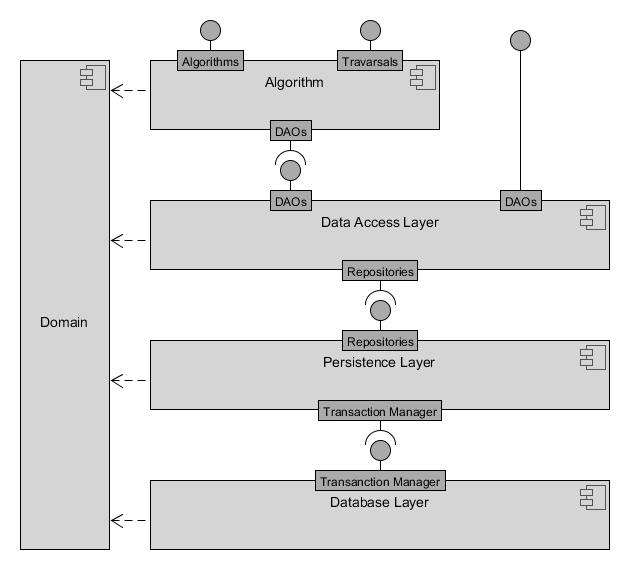
\includegraphics[width=10cm]{figures/connector_modules}
\caption{Upravená architektura modulu Connector}
\label{fig:des-connector}
\end{center}
\end{figure}

\subsubsection{Doménový model}
\label{sec:des_domain}
Jedním z důsledků splývání byznys a persistenční logiky je absence doménového objektového modelu serverové části aplikace. Místo něj je používán obecný model založený na třídách \textit{Vertex} (vrchol) a \textit{Edge} (hrana). Tato reprezentace dat v aplikaci má dva zásadní dopady:

\begin{itemize}
   \item Model je příliš obecný (dokáže pojmout graf jakékoliv struktury, potažmo graf bez definované struktury), datový model metadatového uložiště je ale přesně specifikovaný (diagram \ref{fig:ana-model}) a jeho nedodržení znamená zanesení nekonzistence a tedy riziko selhání aplikace.
   \item Vzhledem k tomu, že zmíněný model poskytuje jako \textit{SPI} dotazovací jazyk \textit{Gremlin} (respektive \textit{API Blueprints}) a to je implementováno \textit{Java} knihovnou pro práci s grafovou databází \textit{Titan}, umožňují instance tohoto modelu přímý přístup do grafové databáze a umožňuje tedy obcházení metod dedikovaných pro práci s grafovou databází.
\end{itemize}

Je evidentní, že tento doménový model není pro navrženou architekturu vhodný, byl tak vytvořen vlastní, \textbf{specifický doménový model}.

Základními omezeními návrhu doménového modelu jsou:
\begin{itemize}
   \item{\textit{Rich model}}: Doménový model je navržen jako tzv. \textit{rich domain model}, obsahuje nejen definice entint a jejich parametrů, ale také základní logiku, kterou tyto entity a vazby mezi nimi představují.
   \item{\textit{POJO model}}: Doménový model by měl být tvořen pouze \textit{POJO třídami} \footnote{\textit{POJO (Plain Old Java Object)} je označení pro \textit{obyčejný Java objekt}, tedy objekt, který není \textit{J2EE Bean, Spring Bean, Entity Bean,}  atd.}.
   \item{\textit{Model neobsahuje perzistenční logiku}}: Součástí doménového modelu by neměla být perzistenční logika. Toto omezení je v podstatě důsledkem omezení na \textit{POJO} objekty - obsahoval-li by doménový model perzistenční logiku, musel by nutně obsahovat také transakční logiku, která je ale navržna tak (kapitola \ref{sec:des_transactions}), že není realizovatelná pomocí \textit{POJO} objektů. Perzistenční logika je tak realizovaná samostatnou komponentou (kapitola \ref{sec:des_persistence}).
\end{itemize}

\subsubsection{Databázová vrstva}
\label{sec:des_database}
Databázová vrstva slouží pouze pro připojení aplikace do databáze a pro dodání podpory pro externí indexovací nástroje, pokud je potřeba. Základní rozhraní této vrstvy tvoří \textit{TransactionManager}, díky kterému jsou podporovány \textit{deklarativní transakce} ve vyšších vrstvách aplikace a rozhraní reprezentující grafovou databázi\footnote{V případě jazyka \textit{Gremlin 2.x} poskytuje přístup do databáze rozhraní \textit{com.tinkerpop.blueprints.Graph}.} jako vstupní bod pro dotazy do databáze.

Tato funkcionalita je vyčleněna do samostatné vrstvy především kvůli principu separace zájmů. Také v některých případech umožňuje výměnu grafové databáze bez úprav vyšších vrstev - jedná se o případy, kdy je možné obě databáze dotazovat pomocí stejné verze jazyka \textit{Gremlin}.

\subsubsection{Perzistentní vrstva}
\label{sec:des_persistence}
Jak je zmíněno v kapitole \ref{sec:ana_state_of_art}, žádný ze zkoumaných nástrojů pro abstrakci objektově-grafového mapování nevyhovuje požadavkům \textit{Manta Flow} a navržená architektura tak s žádný takový nástroj nepoužívá. Místo toho je navržena vlastní softwarová vrstva, která toto mapování provádí. Tou je právě \textit{Perzistentní vrstva}. Jejím úkolem je poskytnout \textit{API}, které pokryje všechny požadavky na dotazy do grafové databáze (a jeho implementaci). \textit{Perzistentní vrstva} je \textit{uzamčená vrstva} (viz \ref{sec:n-tier}), nemůže tedy být obcházena vyššími vrstvami při přístupu k nižší vrstvě.

\textbf{API je tvořeno sadou \textit{repository} objektů}, které implementují (mimo jiné) \textit{CRUD} operace a jsou inspirovány návrhovým vzorem \textit{Repository pattern} \cite{Dorfmann16}. Pro každou entitu reprezentovanou doménovým modelem existuje jeden \textit{repository} objekt, přičemž každý z těchto objektů obsahuje (pokud je to pro příslušnou entitu relevantní) následující typy metod:

\begin{itemize}
   \item{\textbf{Create}}: Metody slouží pro vytváření nových instancí entit (uzlů a hran) v grafové databázi. Parametrem je samotná instance obsahující parametry uzlu/hrany, interval platnosti uzlu/hrany a pokud existují, tak uzly, které jsou přímímy předky v hiearchii stromu grafových toků (v takovém případě je mezi těmito uzly vytvořena hrana). Například při vytváření nové instance entity \textit{Node} je uzel spojen s rodičovckou instancí entity \textit{Node} a/nebo s instancí entity \textit{Resource}\footnote{Již dříve bylo uvedeno, že graf datových toků ve skutečnosti nesplňuje stromovou strukturu. Je tak například možné, že entita \textit{Node A} bude mít rodičovskou entitu \textit{Node B} a \textit{Resource C}, přičemž \textit{B} a \textit{C} nejsou součástí stejného podstromu grafu datových toků.}.

   \item{\textbf{Find}}: Vstupem \textit{find} metod je jeden nebo více parametrů specifických pro danou entitu, přičemž kombinací těchto parametrů musí být vždy unikátně identifikovatelná maximálně jedna instance entity. Příkladem může být (jazykem \textit{Gremlin} generované) id instance (jakékoliv entity), název entity \textit{Resource}, nebo plně kvalifikované jméno entity \textit{Node}. Metoda pak vrací nalezenou instanci entity - pokud existuje.

   \item{\textbf{Update}}: Operace \textit{update} je u většiny entit redukována na úpravu intervalu platnosti entity, respektive na úpravu konce tohoto intervalu (začátek intervalu je po vytvoření instance neměnný). Ten je upravován při \textit{updatu} (ať už úplném, nebo inkrementálním) metadatového uložiště operací \textit{merge}. V případě, že se jedná o inkrementální \textit{update}, je možné operaci volat s parametrem definujícím, že operace bude rekurzivní - bude uplatněna na celý podstrom entity (včetně entity samotné). Pokud by úpravou konce intervalu platnosti došlo k situaci, že by instance entity nebyla platná již v žádné revizi, je instance smazána pomocí operace \textit{delete}.

    U entity \textit{Flow} je navíc možné přidávat uživatelsky definované parametry entity. Tyto parametry nejsou součástí doménového ani datového modelu aplikace a nejsou ani využívány žádnými algoritmy byznys logiky aplikace. Všechny ostatní parametry (všech entit) jsou jasně definované v doménovém i datovém modelu aplikace, jsou nastavovány při vytváření instance entity operací \textit{update} a dále jsou neměnné.

   \item{\textbf{Delete}}: Metody typu \textit{delete} maže entity v grafové databázi bez ohledu na jejich interval platnosti. Operace může být (stejně jako operace \textit{update}) rekurzivní.

   \item{\textbf{Get*}}: Metody typu \textit{get*} slouží k dohledání entit, které jsou s vstupní entitou propojeny. Příkladem může být dohledání potomků (či předků) entit \textit{Node} a \textit{Resource}, dohledání parametrů (entit \textit{Attribute}) entity \textit{Node}, nebo dohledání entit, které jsou s vstupní entitou propojeny hranami \textit{Flow}, nebo \textit{MapsTo}.

   Metody typu \textit{get*} mají zpravidla další argumenty, které slouží k filtrování dohledávaných entit. Pokud kombinace těchto argumentů vytváří unikátní identifikaci instancí entity v rámci kontextu dotazu (vstupní entity), tak je podle jmenné konvence součástí názvů metody jednotné číslo dohledávané entity (například metoda \textit{getChild}). Pokud argumenty unikátní identifikátor netvoří, je součástí názvu metody množné číslo dohledávané entity (například metoda \textit{getChildren}).

   \item{\textbf{Index Search}}: Zatímco ostatní metody pro dotazování dat z grafové databáze (\textit{find, get*, query}) implicitně využívají existujících interních indexů grafové databáze (a perzistentní vrstva od nich tak odstiňuje vyšší vrstvy), pro využítí externích indexů (v případě \textit{Manta Flow} se jedná o \textit{Apache Lucene}) je nutné definovat vlastní metody. Argumenty těchto metod jsou definovány přesně dle definic těchto externích indexů tak, aby byl plně využit jejich potenciál. Případné další filtrování výsledků těchto dotazů (na základě parametrů neobsažených v externích indexech) tak musí probíhat již v komponentách realizujících byznys logiku aplikace.

   \item{\textbf{Query}}: Metody typu \textit{query} slouží k obecnému dotazování entit. Argumenty těchto metod mohou být filtry  na libovolné parametry entit, včetně parametrů entit s nimi spojenými (hranami a uzly). Na základě těchto argumentů je vygenerovaný databázový dotaz, jehož součástí je uplatnění všech těchto filtrů - jedná se tak o výrazně efektivnější přístup než je například dotázání všech uzlů z grafové databáze a jejich následné filtrování ve vyšších vrstvách aplikace. Jedná se o nejobecnější nástroj, který API pro dotazování dat z grafové databáze nabízí.
\end{itemize}

% struktura
Samotná perzistentní vrstva je dále rozčleněna na komponenty (viz diagram \ref{fig:des-persistence}). Účelem tohoto rozdělení je striktní oddělení \textit{API} komponenty a jeho implementace. Aplikace \textit{Manta Flow} používá pro správu závislostí nástroj \textit{Maven}\footnote{\url{https://maven.apache.org/}}, u jednotlivých modulů je tak definovány, jakým způsobem by měly být referencovány. Analogicky s tímto návrhem by měly být navržena také další vrstvy, které mohou být v budoucnosti do architektury přidávány. Jsou definovány tři moduly:

\begin{itemize}
   \item{\textit{API}}: Modul definuje rozhraní pro používání perzistentní vrstvy. Vyšší vrstvy využívající perzistenční vrstvu by měly referencovat právě tento modul.
   \item{\textit{Test}}: Modul obsahuje třídy s definicemi testů pokrývajících funkcionalitou \textit{API} - bez využití jakékoliv implementace \textit{API}. Jednotlivé implementace \textit{API} potom tyto testy implementují (poskytují implementaci \textit{API}), čímž je zajištěno, že je vždy testováno chování \textit{API}, a ne jen specifické detaily poskytnutých implementací. Modul závisí na modulu \textit{API}.
   \item{\textit{Implementace}}: Modul obsahující implementace vrstvy. Vyšší vrstvy využívající perzistenční vrstvu by tento modul měly referencovat, pouze ale s parametrem \textit{scope=provided}. To zaručí, že není možné v kódu komponent používajích perzistenční vrstvu používat třídy, které jsou součástí této třídy a je tak zaručeno, že definované \textit{API} není obcházeno. Modul je závislý na modulu \textit{API}, modulu \textit{Test} (\textit{scope=test}) a na modulech představují \textit{API} nižší vrstvy.
\end{itemize}

\begin{figure}
\begin{center}
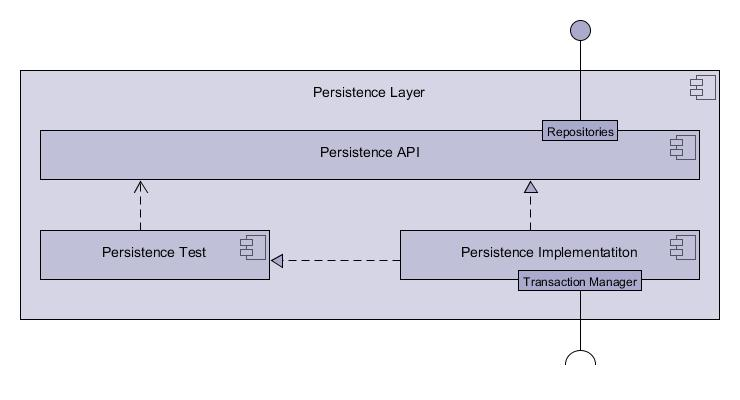
\includegraphics[width=12cm]{figures/persistance_module}
\caption{Struktura perzistenční vrstvy}
\label{fig:des-persistence}
\end{center}
\end{figure}

\subsubsection{Vrstva datového přístupu}
\label{sec:des_data_access}
Vrstva datového přístupu je nejbližší vyšší vrstva perzistentní vrstvy, jejíž funkcionalitu rozšiřuje o kontrolu oprávnění uživatele na dotazovaná data\footnote{Grafové databáze typicky neumožňují definovat oprávnění jednotlivých uživatelů tak, jak je tomu například u \textit{RDBMS} databází.}. \textit{API} této vrstvy kopíruje \textit{API} perzistentní vrstvy, přičemž každou metodu dotazující data\footnote{Kontrola oprávnění není nutná ve všech případech. Existuje premisa, že pokud má uživatel oprávnění na instanci entity, pak musí mít nuntě oprávnění na všechny předky této instance v hiearchii grafu datových toků.} rozšiřuje o definici strategie, pomocí které dojde k validaci oprávnění uživatele. Z výsledků metod perzistentní vrstvy jsou tak v závislosti na zvolené strategii kontroly oprávnění případně odstraňována data, na která uživatel nemá oprávnění. Vrstva datového přístupu vrstva je \textit{uzamčená vrstva}.

\subsubsection{Algoritmy}
Další vrstva - \textit{Algoritmy} obsahuje funkcionalitu stávajícího modulu \textit{Connector}, respektive jeho částí \textit{Algorithm} a \textit{Traversal}. Jedná se o první vrstvu realizující byznys logiku aplikace (funkcionalita je popsána v kapitole \ref{sec:ana_connector}). Jedná se o \textit{odemčenou vrstvu}, může být tedy obcházena vyššími vrstvami v případě, že chtějí použít přímo \textit{API} vrstvy datového přístupu. Komponentami ve vyšších vrstvách serverové části aplikace jsou \textit{Merger, Viewer, Exporter a Public Api}.


\section{Orchestrace komponent Manta Flow}
\label{sec:des_architecture}
TODO

\section{Možnosti horizontálního škálování aplikace}
\label{sec:des_scaling}
TODO

%%%%%%%%%%%%%%%%%%%%%%%%%%%%%%%%%%%%%%%%%%%%%%%%%
% Vrstvy:
% Algorithm/Traversal layer - vrstva algoritmů a traversalů, resp. "business" v kontextu DAL, neměla by sahat přímo do DB. Tatvo vrstva by možná měla obsahovat ještě sourozence Index (lucene) a DAO (most na operations).


%\subsection{Architektonická omezení}
% Podněty
% - Architektura vyhovující cloudovým požadavkům
%  - žádný filesystem, jen pipes na jiné služby, které mohou filesystem podporovat (lze využívat pouze temp uložiště a sfree buckety)
%  - např jedna služba client, jedna server, jedna grafovka
%  - jak by se řešily veškeré konfigurace

% Škálovatelnost - cloud
% https://acloud.guru/
% https://www.amazon.com/Patterns-Enterprise-Application-Architecture-Martin/dp/0321127420
% https://martinfowler.com/articles/microservices.html
% https://martinfowler.com/tags/application%20architecture.html - Serverless Architectures on AWS
% https://www.youtube.com/watch?v=LAWjdZYrUgI
% AWS Lambda - amazon SaaS (?)
% S3 - cloud storage (?)
% Cloud computing http://nvlpubs.nist.gov/nistpubs/Legacy/SP/nistspecialpublication800-145.pdf
% JPMC GAIA https://www.americanbanker.com/news/unexpected-champion-of-public-clouds-jpmorgan-cio-dana-deasy
% Cloud Awareness ;  OpenStack
